%===============================================================
% Author: Rodolfo Ferro Pérez
% Email: ferro@cimat.mx
% Twitter: @FerroRodolfo
%
% ABOUT COPYING OR USING PARTIAL INFORMATION:
% This document was originally created by Rodolfo Ferro, for
% his talk in DevNightsXVI at Tepache Hacklab.
% Any usage of this document or its contents is granted
% according to the license provided and its conditions.
%===============================================================

\documentclass[usenames,dvipsnames]{beamer}
\usetheme{metropolis} % Use metropolis theme

% Import packages:
\usepackage[many]{tcolorbox}
\usepackage{wrapfig}

\title{Hubot:}
\subtitle{Poniendo ChatOps en tus manos}
\author{Rodolfo Ferro\\{\footnotesize \textcolor{Turquoise}{\textsc{@FerroRodolfo}}}}
\institute{Universidad de Guanajuato\\ CIMAT A.C.\\
\begin{wrapfigure}{r}{0.3\textwidth}
  \vspace{-30pt}
  \begin{center}
    \hspace*{-2cm}
    
\includegraphics[width=0.25\textwidth]{imgs/GCE}
    \hspace*{-4.6cm}
    \vspace{6pt}
    
\includegraphics[width=0.15\textwidth]{imgs/flab}
  \end{center}
\end{wrapfigure}
}
\date{Enero 27, 2018}
\begin{document}
  % Title slide:
  \maketitle

  % Table of contents:
  \begin{frame}{Tabla de contenido}
    \setbeamertemplate{section in toc}[sections numbered]
    \tableofcontents[hideallsubsections]
  \end{frame}

  % First section: Qué es ChatOps
  \section{¿Qué es ChatOps?}
  \begin{frame}[standout]
    \textit{ChatOps es un modelo de colaboración que conecta con gente,
    herramientas, procesos y automatización en un flujo de trabajo
    transparente. }
  \end{frame}

  \begin{frame}[standout]
    \textit{Este flujo conecta el trabajo necesitado, el trabajo
    sucediendo y el trabajo hecho en una locación persistente por personas,
    bots y herramientas relacionadas [1]. }
  \end{frame}

  \begin{frame}{La comunicación como colaboración}
    \begin{center}
      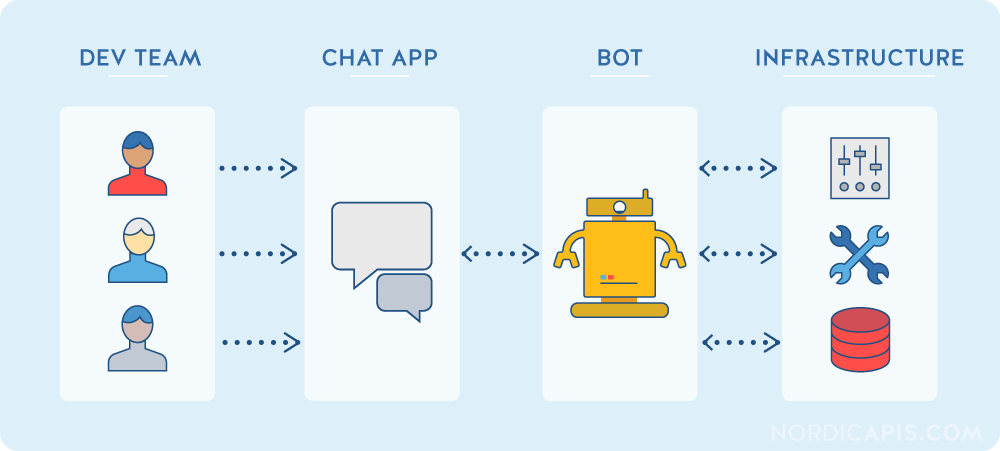
\includegraphics[width=0.8\textwidth]{imgs/chatops}
    \end{center}
  \end{frame}

  % Second section: Dónde se utiliza ChatOps
  \section{¿Dónde se utiliza el ChatOps?}
  \begin{frame}{Caso de estudio: GitHub}
    \begin{itemize}
      \item En 2016 contaban con 603 empleados.
      \item Sólo el 40\% se encontraba basado en San Francisco.
      \item El 60\% se encontraba en el resto del mundo.
      \item Se veían en la necesidad de trabajar de manera remota y asíncrona.
      \item Por la filosofía de GitHub: PRs, Issues, Chat (Campfire).
    \end{itemize}
  \end{frame}

  % Third section: Hubot
  \section{Hubot}
  \begin{frame}{Just kidding!}
    \begin{center}
      
\includegraphics[width=0.4\textwidth]{imgs/bender}
      \textbf{Just kidding!}
    \end{center}
  \end{frame}

  \begin{frame}[standout]
    \begin{center}
      \hspace*{-3cm}
      
\includegraphics[width=1.5\textwidth]{imgs/hubot2}
    \end{center}
  \end{frame}

  % Repo info:
  \begin{frame}[standout]
    
\includegraphics[width=0.3\textwidth]{imgs/Octocat}\\
    Sitio oficial:\\
    {\color{orange} \url{https://hubot.github.com/}}\\
    \vspace*{0.5cm}
    Repositorio oficial:\\
    {\color{orange} \url{https://github.com/hubotio/hubot}}\\
  \end{frame}

  % Fourth section: Desarrollando con Hubot
  \section{Desarrollando con Hubot}
  \begin{frame}{Instalación}
    \begin{itemize}
      \item Instalamos \texttt{NodeJS} y \texttt{yo}.
      \item Hacemos \texttt{npm install -g yo generator-hubot}.
      \item Hacemos \texttt{mkdir hubot \&\& cd \$\_}.
      \item Hacemos \texttt{yo hubot}.
    \end{itemize}
  \end{frame}

  \begin{frame}{Coffescript como lenguaje de desarrollo}
    Si quisiéramos que el bot responda ante la mención de la palabra
    \textit{"tacos"}, la sintaxis correspondiente sería:
    \metroset{block=fill}
    \begin{block}{Ejemplo de función:}
      \hspace{0.0cm}{\color{gray} \texttt{robot.hear }}{\color{Cerulean} \texttt{/}}{\color{LimeGreen} \texttt{tacos}}{\color{Cerulean} \texttt{/}}{\color{LimeGreen} \texttt{i}}{\color{Cerulean} \texttt{, (}}{\color{orange} \texttt{res}}{\color{Cerulean} \texttt{) ->}}\\
      \hspace{0.4cm}{\color{gray} \texttt{res.}}{\color{LimeGreen} \texttt{send }}{\color{Cerulean} \texttt{"TACOS?! YAAAS! WHEN?! WHERE?!"}}\\
      \hspace{0.4cm}{\color{gray} \texttt{}}\\
    \end{block}
    \vspace*{0.5cm}

    Podemos crear diversa cantidad de funciones y guardarlo en un archivo
    de extensión \texttt{.coffee}.
  \end{frame}

  \begin{frame}{Corriendo Hubot}
    Más ejemplos de Hubot pueden ser mostrados a continuación.

    Sólo corremos desde nuestra carpeta con Hubot:\\
    \begin{center}
      \texttt{./bin/hubot}
    \end{center}
  \end{frame}

  % Fifth section: Más allá de ChatOps
  \section{Más allá de ChatOps}
  \begin{frame}{No sólo Hubot}
    \begin{center}
      % \hspace*{-3cm}
      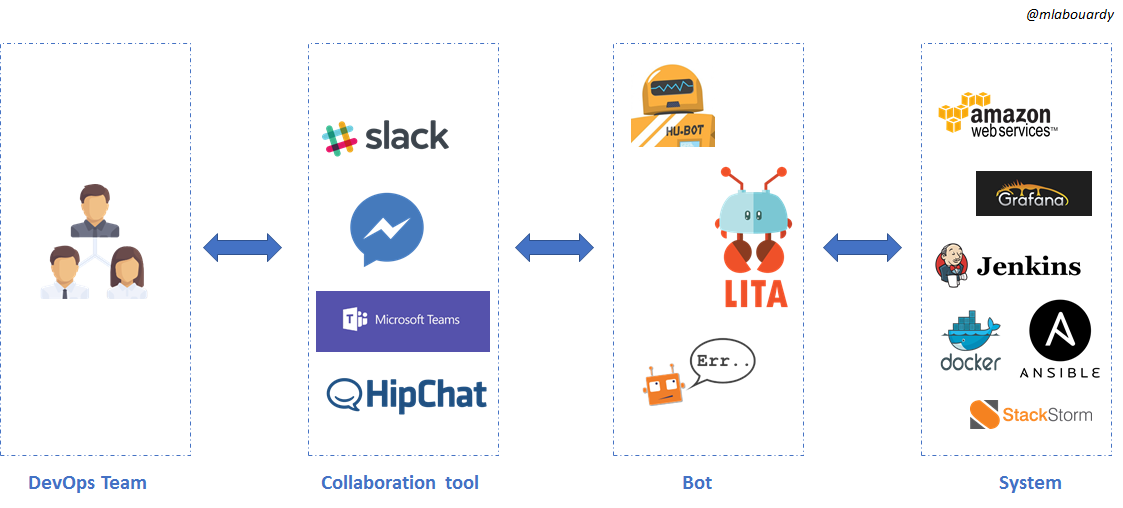
\includegraphics[width=1.0\textwidth]{imgs/chatops2}
    \end{center}
  \end{frame}

  \begin{frame}{Explotemos el potencial de ChatOps}
    \begin{center}
      % \hspace*{-3cm}
      
\includegraphics[width=1.0\textwidth]{imgs/chatops4}
    \end{center}
  \end{frame}

  % Questions
  \begin{frame}[standout]
    ¿Preguntas?
  \end{frame}

  % References
  \begin{frame}{Referencias (I)}
    \begin{enumerate}[{[}1{]}]
      \item Sean Regan, Atlassian Blog.\\
      \textbf{What is ChatOps? A guide to its evolution, adoption, and significance}.\\
      \textit{What is ChatOps? Conversations, put to work},
      disponible en \texttt{https://www.atlassian.com/blog/software-teams/what-is-chatops-adoption-guide}, 2016.
    \end{enumerate}
  \end{frame}

  \begin{frame}{Referencias (II)}
    \begin{enumerate}[{[}3{]}]
      \item StackStorm.\\
      \textbf{What is ChatOps?}.\\
      \textit{What is ChatOps?},
      disponible en \texttt{https://docs.stackstorm.com/chatops/chatops.html}, 2014 - 2018.
    \end{enumerate}
  \end{frame}

  \begin{frame}{Referencias (III)}
    \begin{enumerate}[{[}3{]}]
      \item Eric Sigler, Pager Duty.\\
      \textbf{So, what is ChatOps? And how do I get started?}.\\
      \textit{Help your teams communicate and collaborate better},
      disponible en \texttt{https://www.pagerduty.com/blog/what-is-chatops/}, 2014.
    \end{enumerate}
  \end{frame}

  % Thanks
  \begin{frame}[standout]
    
\includegraphics[width=0.2\textwidth]{imgs/me}\\
    {\color{Turquoise} \textsc{@FerroRodolfo}}\\
    Repositorio de la charla:\\
    {\color{orange} \url{https://github.com/RodolfoFerro/DevNightXVI}}\\
    \vspace*{0.3cm}
    \noindent {\color{white} \rule{0.3\linewidth}{1mm} }\\
    \vspace*{0.3cm}
    ¡Gracias por su atención!
  \end{frame}
\end{document}
